\documentclass{sprawozdanie-agh}


\usepackage[utf8]{inputenc}
\usepackage{listings}
\usepackage{pdfpages}
\usepackage{float}
\usepackage{anyfontsize}
\usepackage{courier}
\usepackage{hyperref}

\lstset{basicstyle=\footnotesize\ttfamily,breaklines=true}
 
\makeatletter 

\begin{document}   

	\przedmiot{Inżynieria oprogramowania}
	\tytul{Dokumentacja}
	\podtytul{„Gdzie jest moje dziecko?”}
	\kierunek{Informatyka, III rok, 2018/2019}
	\autor{Agnieszka Zadworny, Piotr Morawiecki, Tomasz Pęcak, Maciej Bielech}
	\data{Kraków, 7 listopada 2018}

	\stronatytulowa{}

	

	\section{Jak zbudować i uruchomić aplikację webową na "devie"?}

		\subsection{Potrzebne pliki}

			Do poprawnego działania aplikacji potrzebujemy dwóch plików, które nie są udostępnione w repozytorium z uwagi na bezpieczeństwo kluczy prywatnych.
			Są to: \lstinline{/server/config/dev.js} i \lstinline{/server/client/.env.development}.
			 \begin{itemize}
				 \item \lstinline{/server/config/dev.js} zawiera: 
					\begin{lstlisting}
						module.exports = {
							googleClientID: 'googleClientID',
							googleClientSecret: 'googleClientSecret',
							mongoURI: 'mongoDBuri',
							cookieKey: 'cookieKey'
						};
					\end{lstlisting}
				\item \lstinline{/server/client/.env.development} zawiera:
					\begin{lstlisting}
						REACT_APP_GOOGLE_KEY='keyGoogleMapsAPI'
					\end{lstlisting}
			 \end{itemize}

		\subsection{Budowanie i uruchamianie}

		Aby uruchomić aplikację webową musimy pobrać pliki z repozytorium,
		nastepnie zainstalować Node.js. Aby zainstalować Node.js postępujemy według instrukcji na oficjalnej stronie nodejs.org. Przykładowe kroki dla Ubuntu i wersji 11 Node.js:

		\begin{lstlisting}
			curl -sL https://deb.nodesource.com/setup_11.x | sudo -E bash -
			sudo apt-get install -y nodejs
		\end{lstlisting}

		Kolejnym krokiem jest przejście do folderu \lstinline{/server} w projekcie i zainstalowanie potrzebnych bibliotek dla części serwera naszej aplikacji uruchamiając następującą instrukcję:

		\begin{lstlisting}
			npm install
		\end{lstlisting}

		Tą instrukcję uruchamiamy również w folderze \lstinline{/server/client} projektu, aby zainstalować biblioteki wykorzystywane w części klienckiej naszej aplikacji.

		Aby uruchomić współbieżnie serwer i klienta uruchamiamy zdefiniowany skrypt:

		\begin{lstlisting}
			npm run dev
		\end{lstlisting}

	\section{Jak uruchomić aplikację webową na "produkcji"?}

		Aby uruchomić aplikację na produkcji należy przejść do adresu \href{https://kid-tracker.herokuapp.com/}{https://kid-tracker.herokuapp.com/} w przeglądarce wspierającej składnie JavaScript 2017.

		Aby wdrożyć aplikację na produkcję należy zastosować następujące kroki:

		\begin{itemize}
			\item Tomek !!!!!!!!!!!!!!!!!!!!!!!!!!!!!!!!!!!!!!!!!!!!!!!!!!!!!!!!!!!!!!!!!!!!
			\item Zrób
			\item Deployment
		\end{itemize}

	\section{Dokumentacja użytkownika (czyli opis interfejsu - co gdzie i jak można zrobić)}

	\section{Dokumentacje techniczna - podział aplikacji na moduły, architektura, opis API i istotnych interfejsów itp.}

		\subsection{Architektura systemu}
		
		\begin{figure}[H] 
			\centering
			\begin{tabular}{c}
				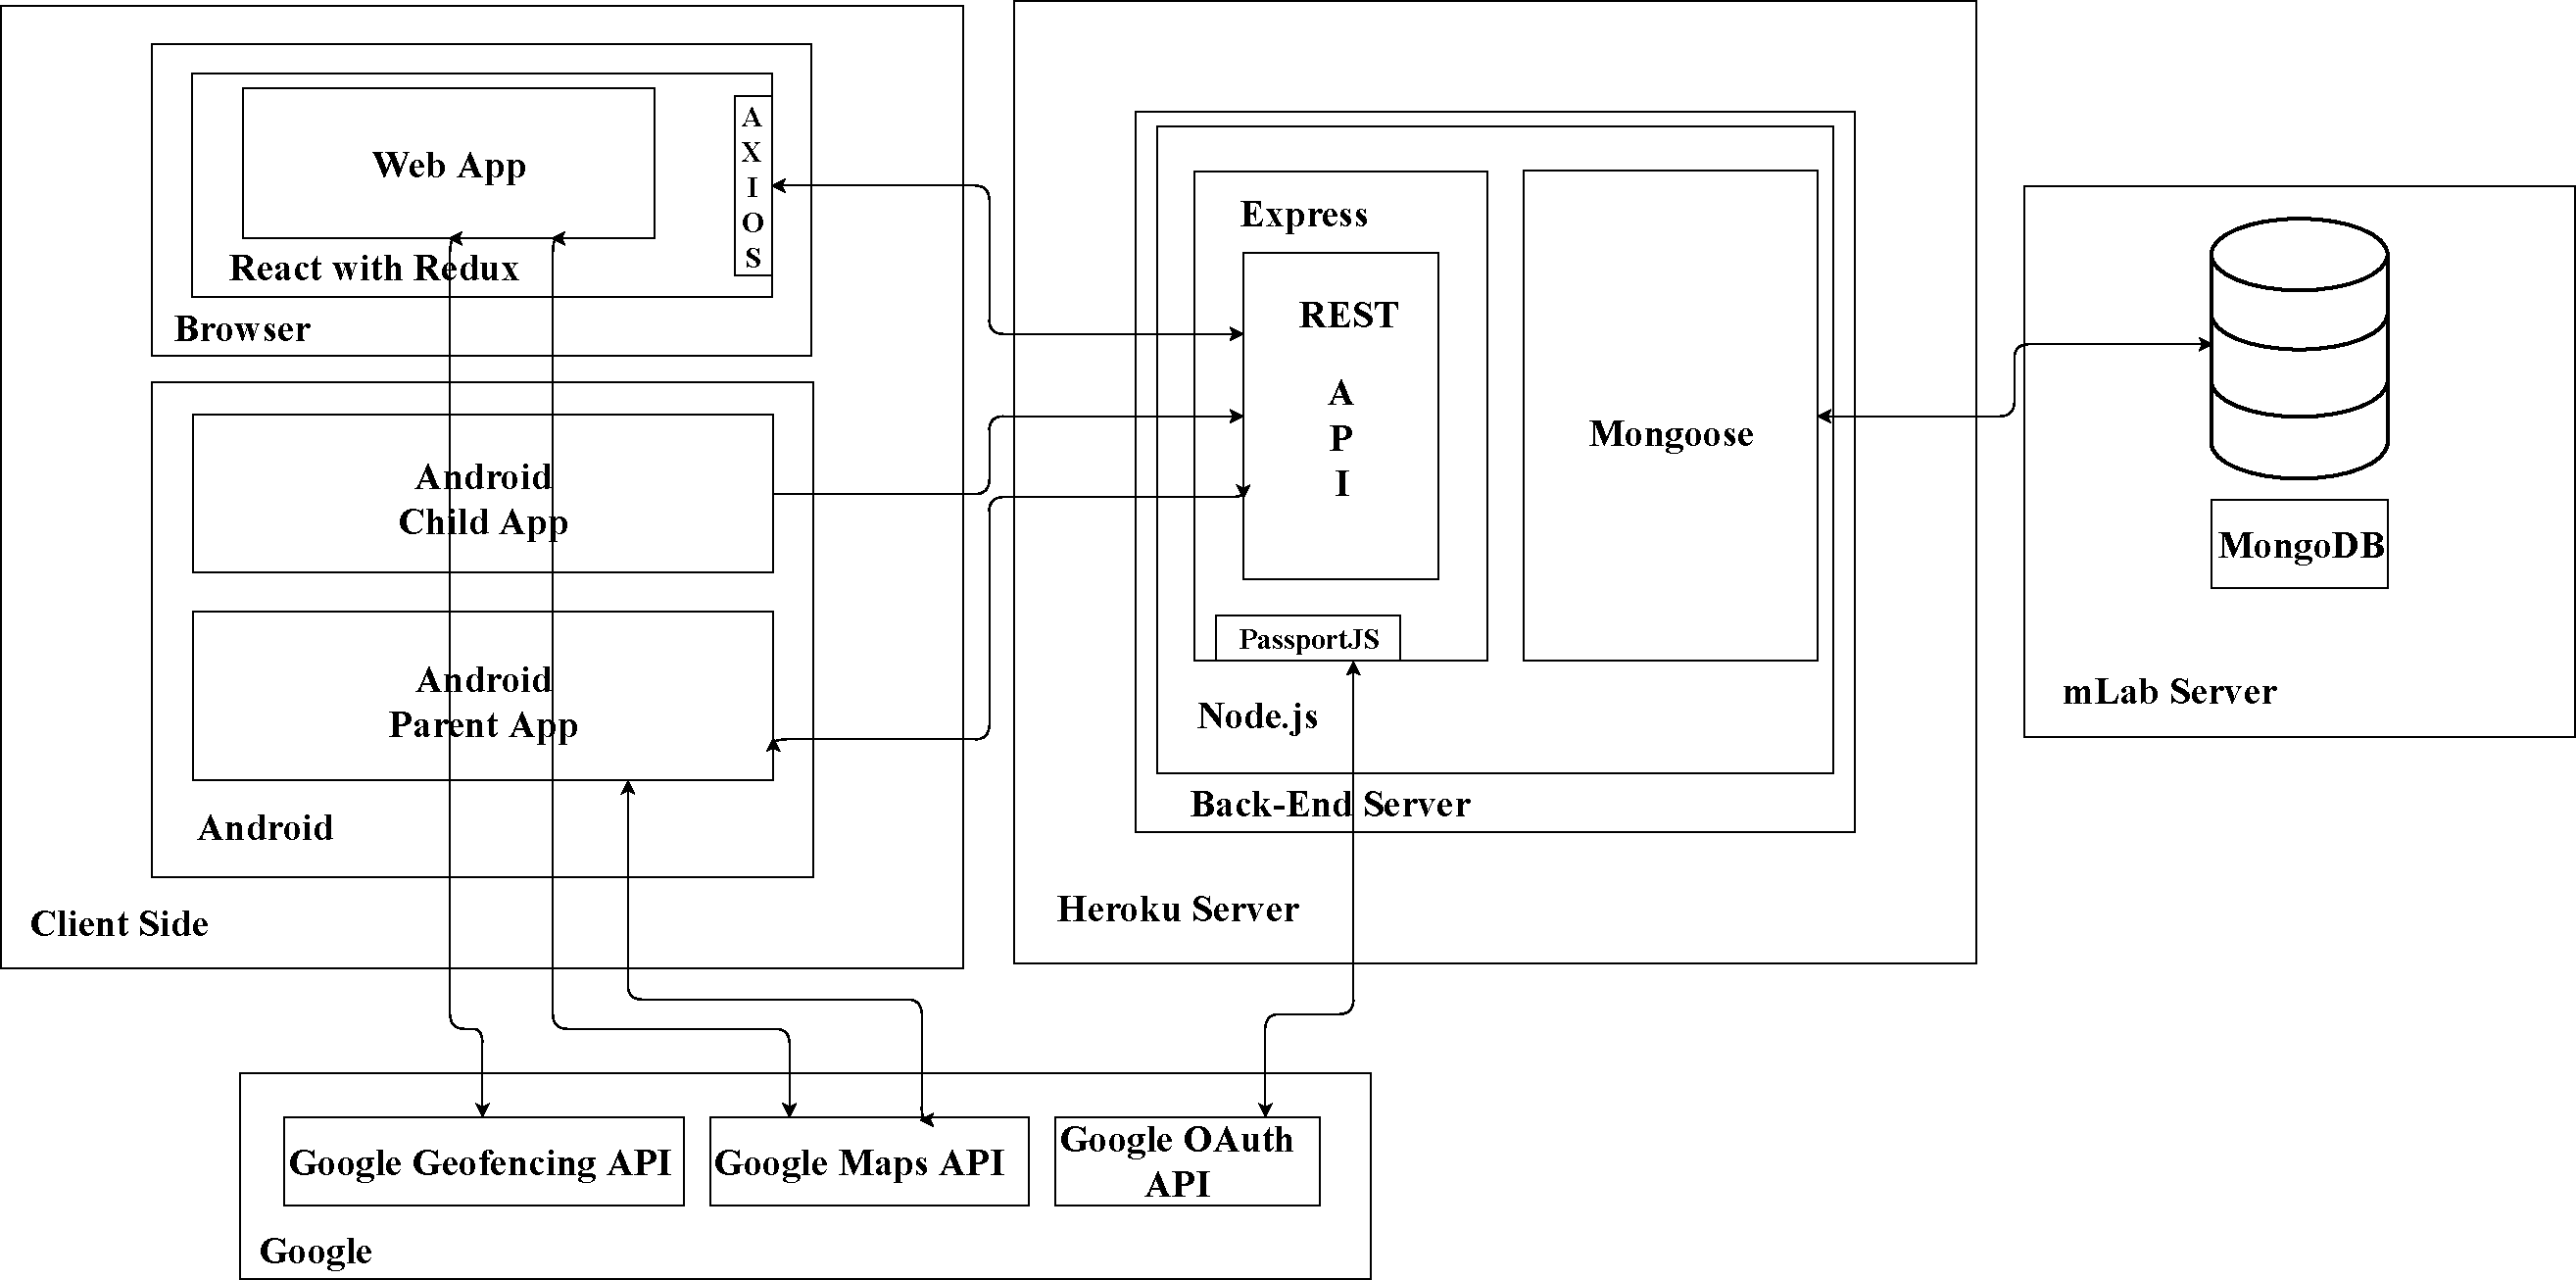
\includegraphics[width=.95\textwidth]{moduly_interfejsy_komunikacyjne}
			\end{tabular} 
			\caption{Architektura, moduły i interfejsy}
		\end{figure}

		\subsection{Frontend aplikacji webowej}

			\subsubsection{Frameworki, biblioteki i technologie}

				\begin{itemize}
					\item React - tworzenie komponentów
					\item Redux - przechowywanie i udostępnianie danych komponentom
					\item axios - tworzenie zapytań do serwera backendowego
					\item reduxThunk - umożliwia asynchroniczne oczekiwanie na odpowiedzi serwera backendowego,
					\item react-router-dom - tworzenie odnośników do różnych komponentów aplikacji
					\item react-google-maps - tworzenie komponentów React odpowiedzialnych za wyświetlanie map Google
					\item semantic-ui-react - tworzenie komponentów z stylizacją semantic ui
				\end{itemize}

			\subsubsection{Podział na foldery}

				\begin{itemize}
					\item actions - akcje wykorzystywane przez redux i reduxThunk do komunikacji frontendu z backendowym serwerem,
					\item components - komponenty React,
					\item reducers - funkcje potrzebne do prawidłowego działania redux
				\end{itemize}

			\subsubsection{Komponenty}

				\begin{itemize}
					\item App - komponent główny aplikacji zawierający BrowserRouter odpowiadający za prawidłowe wyświetlanie komponentów ze względu na ścieżke wpisaną w pole adresu przeglądarki,
					\item Header - komponent zawierający menu, wyświetlany po zalogowaniu się do aplikacji na górze ekranu,
					\item Map - komponent obsługujący wyświetlanie map Google,
					\item folder Landing - zawiera komponenty odpowiedzialne za wyświetlanie ekranu powitalnego, logowania, rejestracji i logowania za pomocą Google,
					\item folder Dashboard - zawiera komponenty wyświetlające aktualnie obowiązujące reguły i wyświetlające mapę z aktualnymi położeniami dzieci,
					\item folder Children - zwiera komponenty wyświetlające powiązane z kontem rodzica dzieci, umożliwia dodawanie nowego dziecka, edycję istniejącego i usunięcie istniejącego,
					\item folder Areas - zawiera komponenty wyświetlające powiązane z kontem rodzica obszary, umożliwia dodawanie nowego obszaru, edycję istniejącego i usunięcie istniejącego,
					\item folder Rules - zawiera komponenty wyświetlające powiązane z kontem rodzica reguły wybranego dziecka, umożliwia dodawanie nowej reguły, edycję istniejącej i usunięcie istniejącej.
				\end{itemize}

		\subsection{API}

			Aplikacja komunikuje się z serwerem poprzez RESTowe API. Aplikacja kliencka użyje systemu axios aby komunikować się poprzez zapytania i odpowiedzi serwera, serwer komunikuje się z bazą danych MongoDB poprzez bibliotekę mongoose.
			
			\begin{itemize}
				\item \textbackslash api\textbackslash current\_user - bieżący zalogowany użytkownik,
				\item \textbackslash api\textbackslash logout - wylogowanie użytkownika,
				\item \textbackslash api\textbackslash googleAuth - logowanie z Googlem,
				\item \textbackslash api\textbackslash register - rejestrowanie nowego użytkownika,
				\item \textbackslash api\textbackslash login - logowanie emailem i hasłem,
				\item \textbackslash api\textbackslash rules - reguły dla bieżącego użytkownika,
				\item \textbackslash api\textbackslash rules\textbackslash create - tworzenie nowej reguły,
				\item \textbackslash api\textbackslash rules\textbackslash update - modyfikacja reguły,
				\item \textbackslash api\textbackslash rules\textbackslash delete - usuwanie reguły,
				\item \textbackslash api\textbackslash areas - areas for current user,
				\item \textbackslash api\textbackslash areas\textbackslash create - tworzenie nowego obszaru,
				\item \textbackslash api\textbackslash areas\textbackslash update - modyfikacja obszaru,
				\item \textbackslash api\textbackslash areas\textbackslash delete - usuwanie obszaru,	
				\item \textbackslash api\textbackslash children - dzieci dla bieżącego użytkownia,
				\item \textbackslash api\textbackslash children\textbackslash create - tworzenie nowego dziecka,
				\item \textbackslash api\textbackslash children\textbackslash update - modyfikacja dziecka,
				\item \textbackslash api\textbackslash children\textbackslash delete - usuwanie dziecka.
			\end{itemize}
		
		\subsection{Diagramy bazy danych}

			\begin{figure}[H] 
				\centering
				\begin{tabular}{c}
					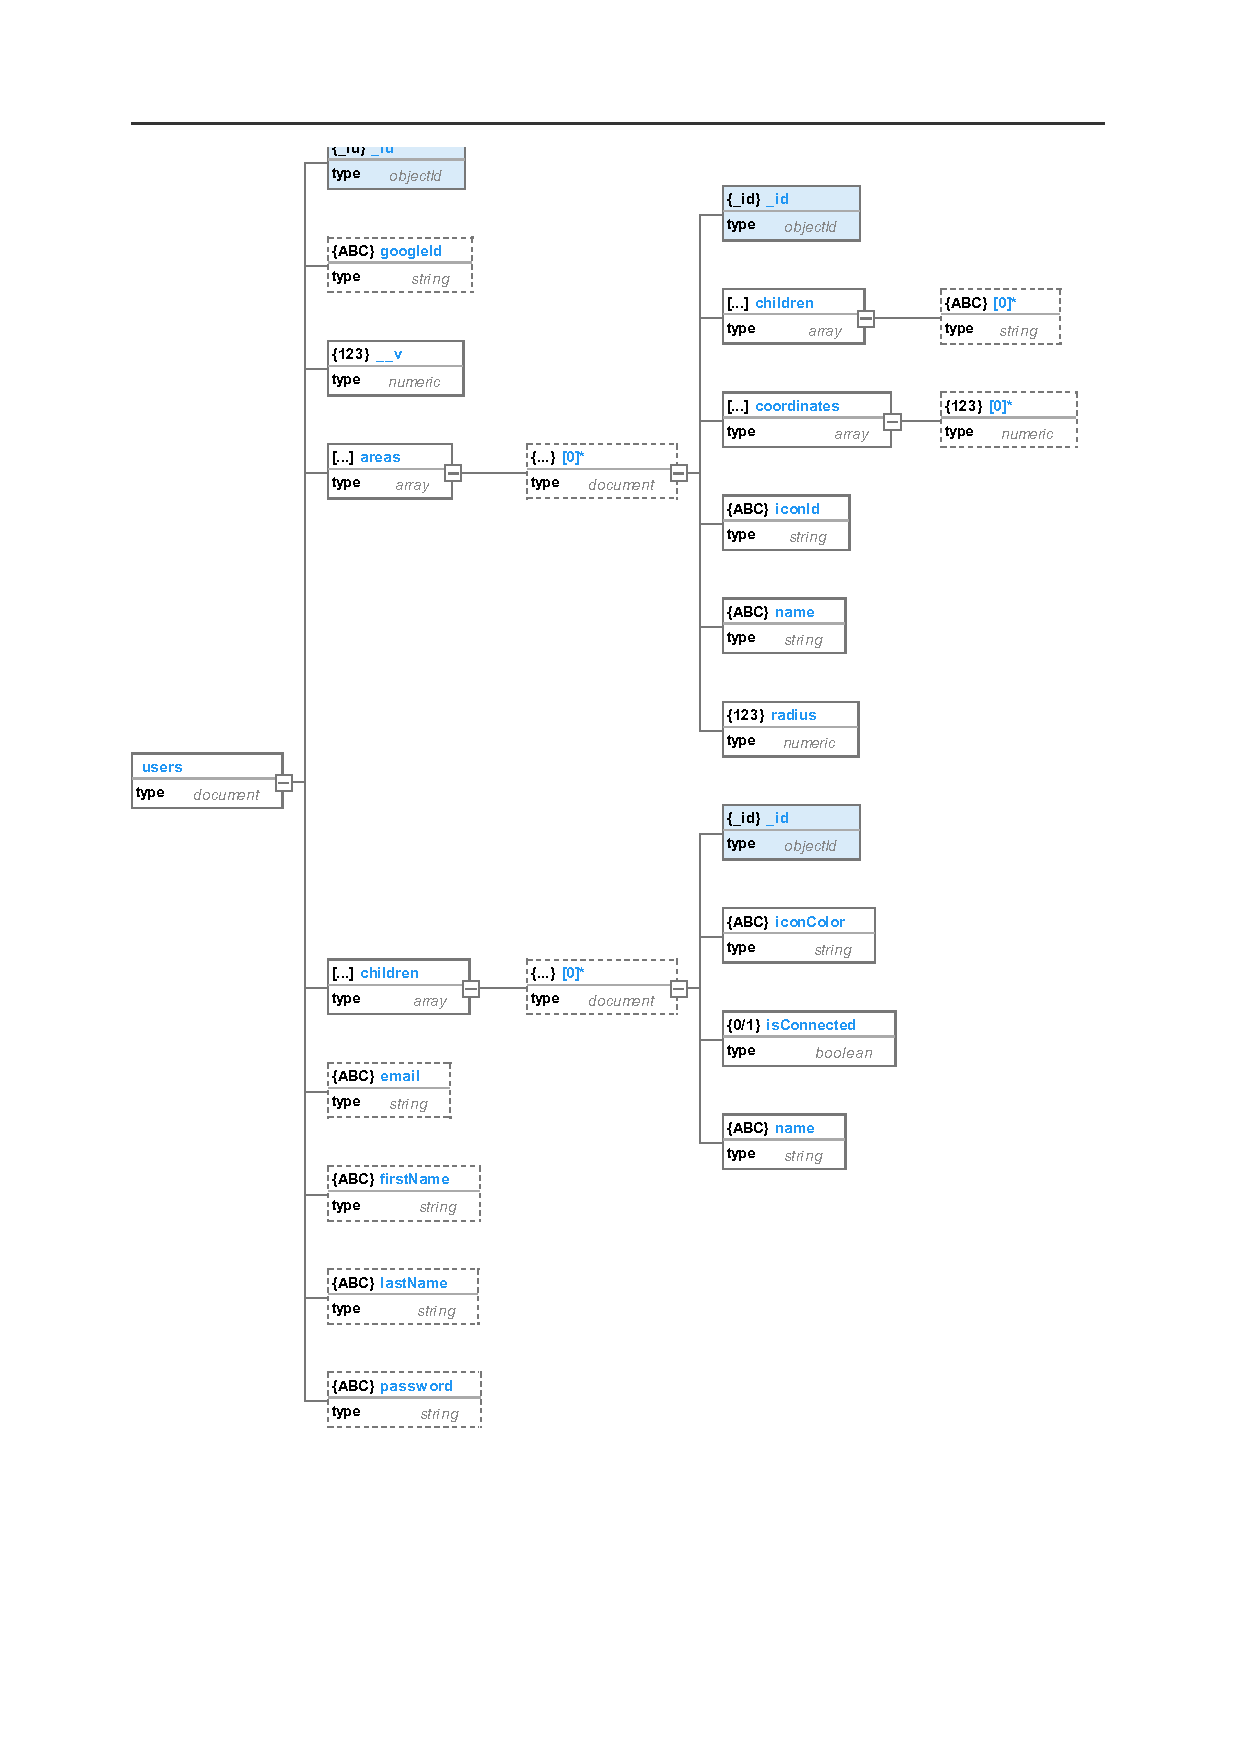
\includegraphics[width=.95\textwidth]{usersDatabase}
				\end{tabular} 
				\caption{Schemat dokumentu użytkownika}
			\end{figure}

			\begin{figure}[H] 
				\centering 
				\begin{tabular}{c}
					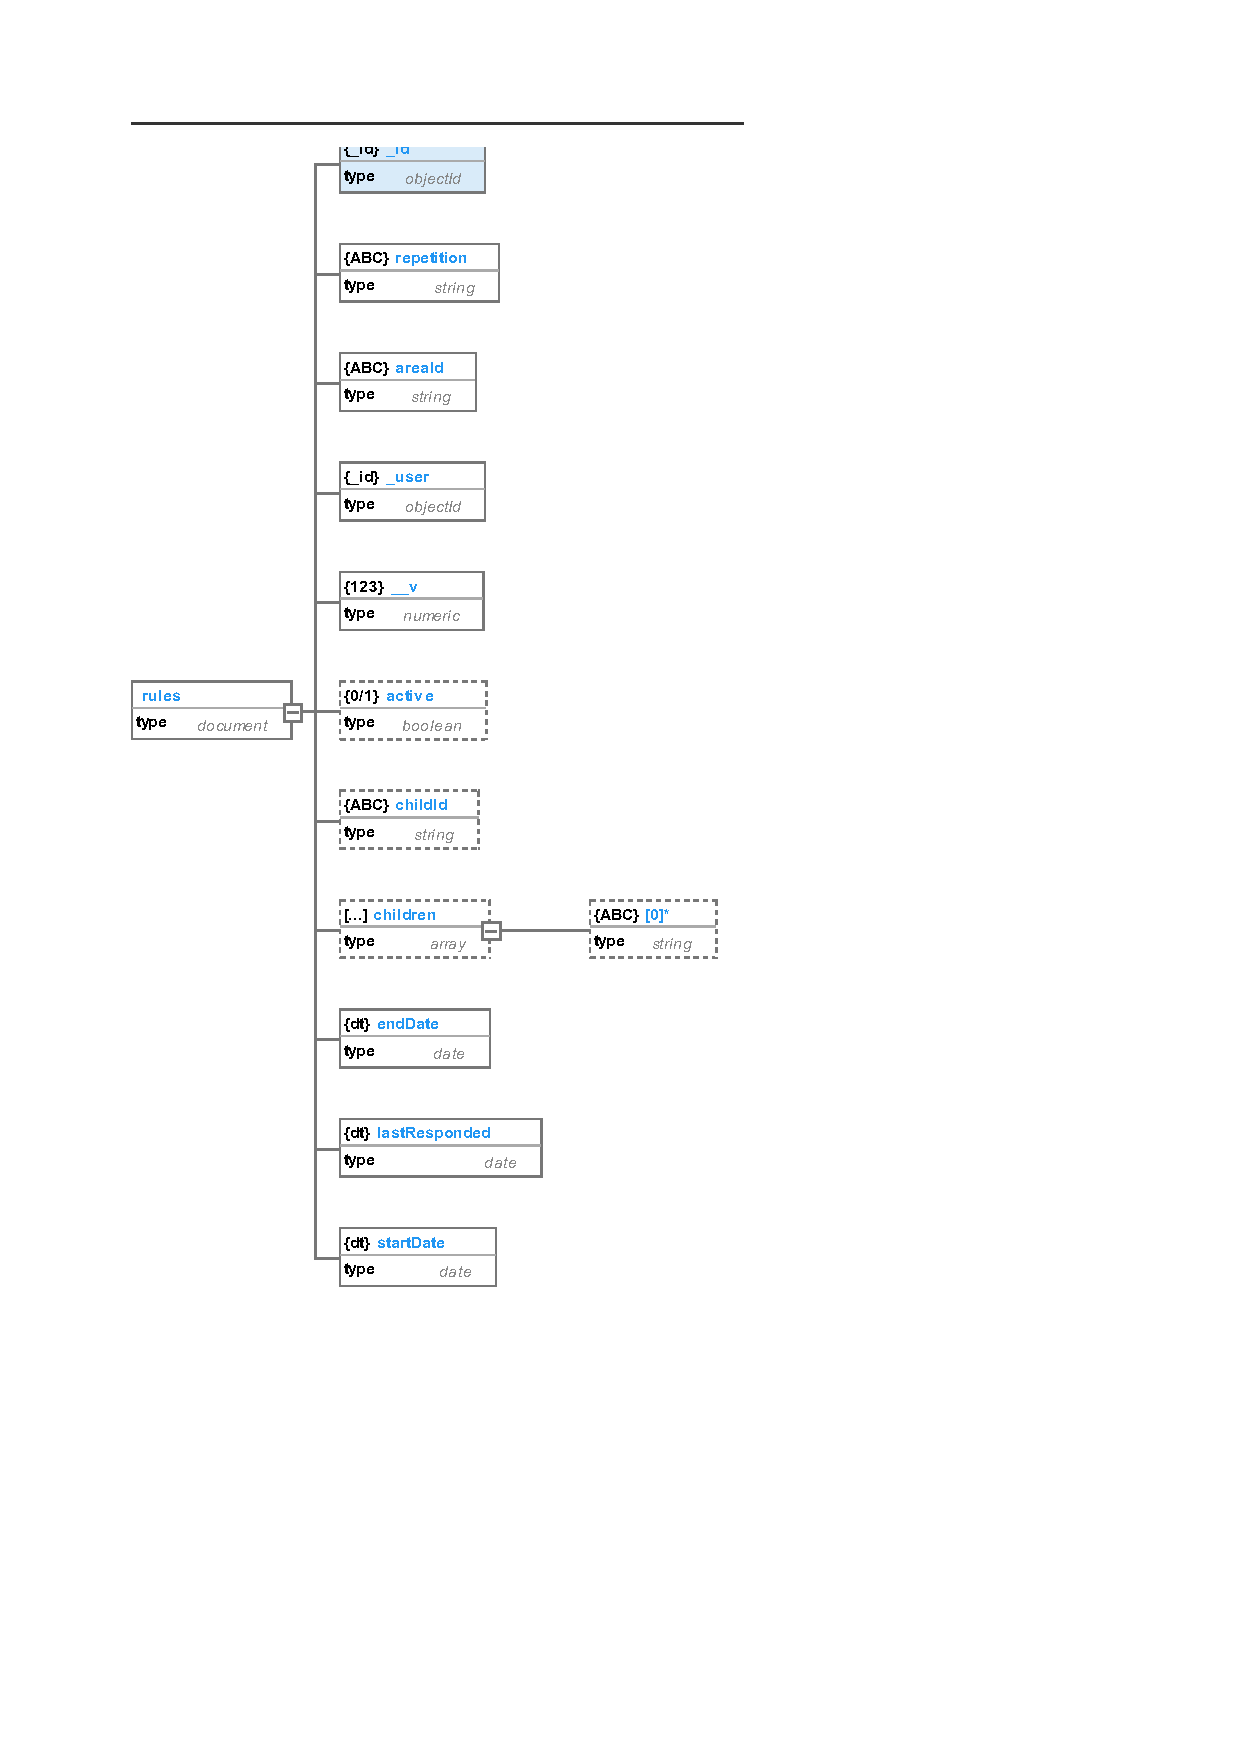
\includegraphics[width=.70\textwidth]{rulesDatabase} 
				\end{tabular} 
				\caption{Schemat dokumentu reguły}
			\end{figure}


	\section{Testy automatyczne (jednostkowe i funkcjonalne) aplikacji}
	
\end{document}